\documentclass{emulateapj}
\submitted{{\it Submitted for publication in ApJ Letters}}
\usepackage{multirow,color,wrapfig,ulem}
\usepackage {graphicx}
\usepackage{graphics}
\usepackage[dvips]{epsfig}
\newcommand{\avg}[1]{\langle{#1}\rangle}  
\newcommand{\nscatt}{\langle N_{\rm  scatt}\rangle}
\newcommand{\ly}{{\ifmmode{{\rm Ly}\alpha~}\else{Ly$\alpha$~}\fi}}
\newcommand{\hMpc}{{\ifmmode{h^{-1}{\rm Mpc}}\else{$h^{-1}$Mpc }\fi}}   
\newcommand{\hGpc}{{\ifmmode{h^{-1}{\rm Gpc}}\else{$h^{-1}$Gpc }\fi}}   
\newcommand{\hmpc}{{\ifmmode{h^{-1}{\rm Mpc}}\else{$h^{-1}$Mpc }\fi}}  
\newcommand{\hkpc}{{\ifmmode{h^{-1}{\rm kpc}}\else{$h^{-1}$kpc }\fi}}  
\newcommand{\hMsun}{{\ifmmode{h^{-1}{\rm
        {M_{\odot}}}}\else{$h^{-1}{\rm{M_{\odot}}}$}\fi}}   
\newcommand{\hmsun}{{\ifmmode{h^{-1}{\rm
        {M_{\odot}}}}\else{$h^{-1}{\rm{M_{\odot}}}$}\fi}}   
\newcommand{\Msun}{{\ifmmode{{\rm {M_{\odot}}}}\else{${\rm{M_{\odot}}}$}\fi}}  
\newcommand{\msun}{{\ifmmode{{\rm {M_{\odot}}}}\else{${\rm{M_{\odot}}}$}\fi}}  
\newcommand{\lya}{{Lyman $\alpha$~}}
\newcommand{\clara}{{\texttt{CLARA}}~}
\newcommand{\rand}{{\ifmmode{{\mathcal{R}}}\else{${\mathcal{R}}$ }\fi}}  
\newcommand{\hs}{{\hspace{1mm}}}  
\newcommand{\kms}{{\ifmmode{{\mathrm{\,km\ s}^{-1}}}\else{\,km~s$^{-1}$}\fi}}
% definition to produce a "less than or similar to" symbol
\def\lsim{~\rlap{$<$}{\lower 1.0ex\hbox{$\sim$}}}
% definition to produce a "greater than or similar to" symbol
\def\gsim{~\rlap{$>$}{\lower 1.0ex\hbox{$\sim$}}}
%@arxiver{fig3.pdf,fig11a.pdf, fig11b.pdf} 
\begin{document}

\title{First estimate of a galaxy rotational velocity from
  its observed Lyman-$\alpha$ line} 
\shorttitle{Rotational velocity from the Lyman $\alpha$ line}

\shortauthors{Remolina-Gutierrez, Garavito-Camargo, Forero-Romero}

\author{ Maria C. Remolina-Gutierrez, Juan N. Garavito-Camargo, Jaime
  E. Forero-Romero}  
\affil{Departamento de F\'{i}sica, Universidad de los Andes, Cra. 1
No. 18A-10, Edificio Ip, Bogot\'a, Colombia}
\email{mc.remolina197@uniandes.edu.co}
\email{jn.garavito57@uniandes.edu.co}
\email{je.forero@uniandes.edu.co}

\keywords{galaxies: high-redshift --- line: formation --- methods:
  numerical ---  radiative transfer} 
\begin{abstract}
First.
\end{abstract}


\section{Introduction}
\label{sec:intro}

Introduction... \\ 
\cite{Garavito14}


\section{Theoretical Background}
\label{sec:theo}


\cite{Garavito14} presented an analytical expresion that approximates
the results for the Lyman-$\alpha$ line morphology for a spherical galaxy
rotating as a solid body.

Ths input parameters of the analytical solution are the optical depth
$\tau_{H}$, the rotational velocity at the sphere's surface $V_{\rm
  max}$ and the angle of view measured from the equatorial plane
(which is perpendicular to the rotational axis) $\theta$. 
A $\texttt{C}$ source code implementation is available in the public
repository associated to this paper.

The main result \cite{Garavito14} is that rotation does have a
noticeable impact on the \ly line morphology.
This impact is two fold. 
First, the rotation axis breaks the spherical symmetry, introducing a
dependence of the line shape with viewing angle.
Second, for increasing rotational velocities and viewing angles off
the rotational axis, the intensity at the line's centers increases;
for sufficiently high rotational velocities the line becomes single peaked. 
 
\section{Results}
\label{sec:results}


\begin{figure}
\begin{center}
  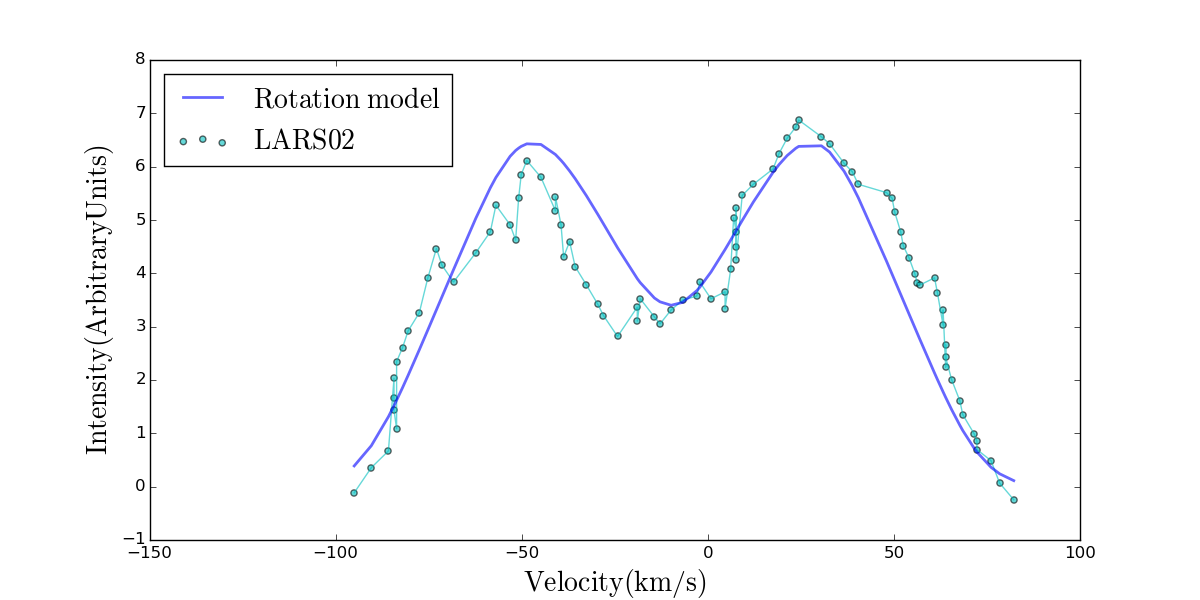
\includegraphics[width=0.5\textwidth]{mcmc.png}
\end{center}
\caption{
    \label{fig:mcmc_result}}  
\end{figure}

\begin{figure*}
\begin{center}
  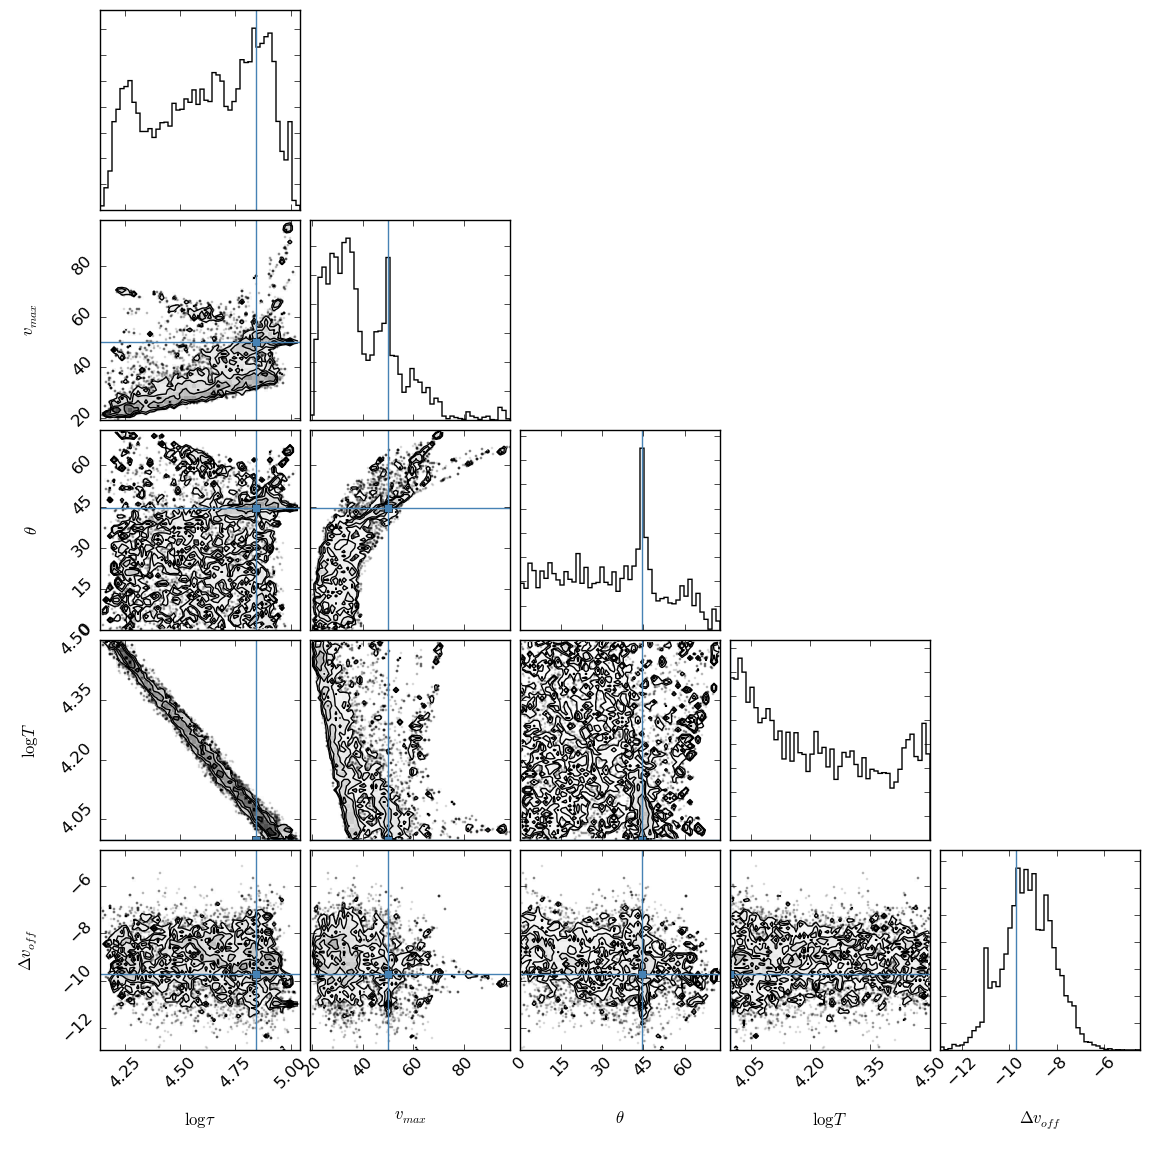
\includegraphics[width=0.7\textwidth]{parameters.png}
\end{center}
\caption{
    \label{fig:mcmc_triangle}}  
\end{figure*}

Results...\\


\section{Discussion}
\label{sec:discussion}

Discussion...\\


\section{Conclusions}
\label{sec:conclusions}

Conclusions...\\


\section*{Acknowledgments}

Acknowledgments...\\



\bibliographystyle{apj}
\bibliography{references}

\end{document}
